\capitulo{5}{Aspectos relevantes del desarrollo del proyecto}

%Este apartado pretende recoger los aspectos más interesantes del desarrollo del proyecto, comentados por los autores del mismo.
%Debe incluir desde la exposición del ciclo de vida utilizado, hasta los detalles de mayor relevancia de las fases de análisis, diseño e implementación.
%Se busca que no sea una mera operación de copiar y pegar diagramas y extractos del código fuente, sino que realmente se justifiquen los caminos de solución que se han tomado, especialmente aquellos que no sean triviales.
%Puede ser el lugar más adecuado para documentar los aspectos más interesantes del diseño y de la implementación, con un mayor hincapié en aspectos tales como el tipo de arquitectura elegido, los índices de las tablas de la base de datos, normalización y desnormalización, distribución en ficheros3, reglas de negocio dentro de las bases de datos (EDVHV GH GDWRV DFWLYDV), aspectos de desarrollo relacionados con el WWW...
%Este apartado, debe convertirse en el resumen de la experiencia práctica del proyecto, y por sí mismo justifica que la memoria se convierta en un documento útil, fuente de referencia para los autores, los tutores y futuros alumnos.

%Despliegue continuo - direccion de app en heroku. Sistema gratuito sirve para validar, pero no para explotar
%Diseño extensible
%Framework vaadin
%No responsive

%Comparacion de tfgs en la ubu, captura dde pantalla con comparativa tfg
Este capítulo recoge los aspectos más relevantes del ciclo de vida del proyecto y justifica los caminos que se han tomado durante el desarrollo. Se menciona el motivo de elección del proyecto, el modelo de ciclo de vida utilizado, una breve explicación de los aspectos de configuración del proyecto y el flujo de trabajo.

\section{Motivación de la elección y relación con asignaturas}

La elección de este trabajo fue motivada por su relación con la asignatura de \textit{Desarrollo Avanzado de Sistemas Software}. En esta se enseña como desarrollar software de calidad mediante el proceso de \textit{Administración de la calidad}, en la cual una de las actividades es el control de calidad. Este control se puede llevar a cabo mediante un proceso de medición. 

En este proyecto se han elegido métricas ya definidas para llevar un control sobre el ciclo de vida de uno o varios proyectos. Esto permite comprender el proceso de desarrollo, evaluarlo respecto a lo que se había planeado, predecir si los planes van por buen camino e identificar los defectos y mejorar la calidad del proceso. Además, esto ha podido ser comprobado, puesto que las mediciones realizadas por el software creado en este proyecto han servido para comparar este proceso con procesos de otros trabajos de fin de grado para saber si la evolución del proyecto era la adecuada.

Este proyecto tiene más relación con la asignatura de \textit{Desarrollo Avanzado de Sistemas Software} pero también se han tomado referencias e ideas de las siguientes materias: 
\begin{itemize}
	\tightlist
	\item De \textit{Estadística} el cálculo de cuartiles para calcular los valores umbrales de las métricas.
	\item De las asignaturas de \textit{Ingeniería del Software} y \textit{Análisis y Diseño de Sistemas}, todo lo relacionado con el ciclo de vida del software, el análisis de los requisitos y el modelado del sistema (diagramas de clases, diagramas de casos de uso, etc).
	\item De \textit{Interacción Hombre/Máquina}  el diseño de la interfaz y las características que este debería alcanzar como usabilidad, la facilidad de aprendizaje, simplicidad, adaptabilidad, etc.
	\item De \textit{Gestión de Proyectos} mayoritariamente el modelo de ciclo de vida del software: Scrum.
	\item De \textit{Diseño y Mantenimiento del Software} el uso de patrones de diseño para mejorar la calidad de código y mantener los principios SOLID  \footnote{Single responsability, Open/Closed, Liskov substitution, Interface segregation, Dependency inversion} y de \textit{Desarrollo Avanzado de Sistemas Software} la naturaleza del trabajo, las revisiones automáticas de calidad de código por medio de métricas y la importancia de la refactorización al detectar defectos de diseño.
	\item \textit{Validación y Pruebas} en la construcción de la batería de pruebas.
	\item \textit{Sistemas Distribuidos} ha ayudado en el uso de Maven y en la construcción de una aplicación web.
	\item \textit{Metodología de la Programación} y \textit{Estructuras de Datos} han contribuido en cuanto a la construcción de una aplicación en un lenguaje Orientado a Objetos.
\end{itemize}

\section{Modelo de ciclo de vida}

Tras la elección del proyecto se acordó definir una evolución que siga las bases del modelo \textit{\textbf{Scrum}}. Tomando un proceso de desarrollo incremental con revisión de las iteraciones cada dos semanas, la duración de un sprint. Estas revisiones se realizaban por medio de reuniones que constaban de dos partes:
\begin{description}
	\item [Revisión del sprint:] Se revisa el incremento generado como resultado del sprint, se describen los problemas que hubo durante su desarrollo y se plantean mejoras sobre el incremento (se puede modificar la pila del producto o \textit{product backlog} \footnote{Lista de requisitos de usuario que, a partir de la visión inicial del producto, crece y evoluciona durante el desarrollo \cite{noauthor_scrum_2019}}) y soluciones a estos problemas.
	\item [Planificación del siguiente sprint:] Se definen las tareas que se deben ejecutar durante el siguiente sprint. Estas tareas en \textit{Scrum} se recogen en la pila del sprint o \textit{sprint backlog}.
\end{description}

Según la naturaleza de los sprints, en el proceso del desarrollo se pueden diferenciar varias etapas:
\begin{itemize}
	\item  Una primera etapa de \textbf{investigación} de las herramientas que se utilizarán durante el proceso y de \textbf{configuración} del entorno de desarrollo.
	\item En la segunda etapa se aprecian tareas de \textbf{diseño e implementación} de la parte lógica de la aplicación. Se diseña el framework de conexión a forjas de repositorios, se implementa el framework descrito en \textit{Soporte de Métricas con Independencia del Lenguaje para la Inferencia de Refactorizaciones}  \cite{marticorena_soporte_2005} para el cálculo de métricas y se diseñan los modelos de datos que serán utilizados por la aplicación.
	\item Durante la segunda etapa se apreció que se debía facilitar el \textbf{flujo de trabajo}, la comunicación entre tutor y alumno y facilitar las reuniones de revisión y planificación del sprint. Esto duro un sprint y se realizaron tareas como:
		\begin{itemize}
			\item Configurar la gestión del proyecto con Maven \footnote{Gestor de proyectos software que ayuda en la construcción del proyecto, la generación de documentación, la generación de informes, la gestión de dependencias, la integración con un sistema de control de versiones, etc.}
			\item Configurar los procesos de integración y despliegue continuo (CI/CD) con GitLab. En estos procesos se realizan actividades automáticamente cada cierto tiempo o cada vez que se realice algún cambio. Ejemplos de estas actividades serían: construir software (\textit{build}), realizar pruebas y revisar su cobertura, desplegar la aplicación en caso de que se trate de una aplicación web, revisar la calidad, etc.
			\item Realizar pruebas unitarias con JUnit y automatizar su ejecución gracias a Maven y los \textit{pipelines} \footnote{Definen las actividades de los procesos de CI/CD y las fases y el entorno en las que se ejecutarán} de GitLab.
			\item Configurar revisiones automáticas de calidad y de cobertura de las pruebas gracias a Maven, Codacy, JaCoCo y GitLab.
			\item Configurar un entorno en Heroku donde poder desplegar la aplicación entre las actividades de CI/CD y así poder ser revisada por el tutor fácilmente.
			\item Configurar badges \footnote{Son placas que aportan información rápida sobre el estado del proyecto en ciertos aspectos como la cobertura, la calidad de código o el estado del proceso de CI/CD} para representar el estado del proyecto en cuanto a calidad de código, cobertura, despliegue y los trabajos de CI/CD.
		\end{itemize}
	\item Etapa  de diseño e implementación de la \textbf{interfaz gráfica} y \textbf{mejora de funcionalidades}. A menudo, estas mejoras precisaban de modificaciones en la parte lógica de la aplicación.
	\item Etapa de \textbf{documentación} en la que se escribe la memoria y los anexos. También se preparan videotutoriales y manuales de usuario.
\end{itemize}

Para más detalles se puede consultar el \textit{Anexo A - Plan de Proyecto Software}. En este se muestra más información sobre estos sprints y el ciclo de vida del proyecto.

\section{Gestión del proyecto}

En esta sección se exponen y se justifican las principales decisiones que se han tomado en cuanto a la configuración del proyecto.

\subsection{Aplicación web}

Para alcanzar los objetivos del proyecto se ha decidido implementar una aplicación web. La principal diferencia es que no se instala en un equipo local sino que se accede a la aplicación desde un navegador web, después de que esta haya sido desplegada en un servidor. Esto tiene varias ventajas: 
\begin{itemize}
	\tightlist
	\item El usuario no necesita instalar la aplicación y puede acceder a ella directamente desde el navegador, esto evita costes de tiempo y de recursos del computador.
	\item  Portabilidad. Es posible que una aplicación de escritorio no pueda ser instalada en ciertos computadores debido a los recursos de los que disponen, el sistema operativo u otros factores. Una aplicación web solo depende del navegador que tenga instalado el computador y, normalmente, puede tener varios instalados. Además, se ha comprobado la portabilidad de navegador y la aplicación funciona en los principales navegadores: Mozilla Firefox, Microsoft Edge, Internet Explorer, Google Chrome y Opera.
	\item Actualizaciones. Para actualizar una aplicación web, el usuario final no tiene que instalar la actualización. Sino que habrá un periodo de mantenimiento de aplicación, normalmente muy corto y fuera de horario de uso, en el que ningún usuario podrá acceder a la aplicación. Después de este periodo, todos los usuarios dispondrán de la actualización.
\end{itemize}

\subsection{Java 11}

El proyecto se iba a desarrollar en Java desde el principio, era uno de los requisitos no funcionales iniciales. La elección de la versión fue uno de los temas que se discutieron al inicio del proyecto. Java 8 era la versión más conocida y la más estable, pero recientemente había surgido la versión 11 de Java. 

Se escogió la versión 11, por ser la más reciente \footnote{Actualmente, la versión Java SE 12.0.2 es la más reciente}. Esto supuso un estudio de las versiones que se debían utilizar de las herramientas que requieren de Java, como Tomcat \footnote{Para desplegar aplicaciones con Java 11 se requiere de la versión 9.0.x de Tomcat} y algunas otras configuraciones. Por ejemplo, se tuvo que configurar el fichero pom.xml del proyecto para que Maven compile en la versión 11 de Java:

\begin{minipage}{\linewidth}
{\tiny
\begin{lstlisting}[breaklines]
...
<properties>
	<project.build.sourceEncoding>UTF-8</project.build.sourceEncoding>
	<project.reporting.outputEncoding>UTF-8</project.reporting.outputEncoding>
	<java.version>11</java.version>
</properties>
...
<build>
...
	<plugins>
		<plugin>
			<groupId>org.apache.maven.plugins</groupId>
			<artifactId>maven-compiler-plugin</artifactId>
			<configuration>
				<source>${java.version}</source>
				<target>${java.version}</target>
			</configuration>
			<version>3.8.0</version>
		</plugin>
		<plugin>
			<groupId>org.apache.maven.plugins</groupId>
			<artifactId>maven-war-plugin</artifactId>
			<version>3.2.2</version>
		</plugin>
		...
	</plugins>
	...
</build>
...
\end{lstlisting}
}
\end{minipage}

Y en Eclipse IDE habría que añadir manualmente el JRE desde la ventana Window/Preferences, como se muestra en la Fig. \ref{fig:M5_Eclipse_Java11}.

\imagen{M5_Eclipse_Java11}{Añadir Java 11 a Eclipse}

Sin embargo, tampoco se trabajó demasiado con las nuevas funcionalidades que trae Java 11, ya que ha sido posible compilar el artefacto final con Java 1.8 y solo han hecho falta dos pequeños cambios:
\begin{itemize}
	\item De la versión 11 se ha utilizado el método \textit{isBlank()} de la clase \textit{String} \footnote{\url{https://docs.oracle.com/en/java/javase/11/docs/api/java.base/java/lang/String.html}}. Se diferencia de \textit{isEmpty()} en que no comprueba la longitud de la cadena y devuelve \textit{true} si es 0. Sino que devuelve \textit{true} si la longitud es 0, o si no es 0 pero todos los caracteres de la cadena son espacios en blanco.
	\item De la clase \textit{java.util.Optional} \footnote{\url{https://docs.oracle.com/en/java/javase/11/docs/api/java.base/java/util/Optional.html}}, soportada desde la versión 1.8, se utiliza la función \textit{orElseThrow()}, que se soporta desde la versión 10, por tanto habría que buscar una alternativa para pasar a la versión 1.8. La versión 11 trae a esta clase la función \textit{isEmpty()}.
\end{itemize}

Para saber más sobre las novedades de Java 11 es recomendable leer `\textit{JDK 11 Release Notes}' \cite{noauthor_jdk_nodate}. También hay un artículo que explica las principales diferencias entre Java 8 y Java 11 llamado `\textit{De Java 8 a Java 11, ¿aún no te has migrado?}' \cite{hoyo_java_2019}.

\subsubsection{Trabajo con streams de Java}

Desde Java 1.8 se puede trabajar con Streams. En este proyecto se ha dado gran uso de ellos ya que facilitan enormemente procesar grandes colecciones de datos. Estos permiten \textbf{filtrar} datos de una colección mediante un predicado, \textbf{ordenar} los datos mediante un comparador, \textbf{mapear} o \textbf{reducir} los datos mediante alguna función y \textbf{almacenarlos} en algún tipo de colección mediante un colector. El mapeo asocia cada dato del stream con un nuevo elemento, por ejemplo, de cada número de una colección numérica obtenemos su potencia de dos. Y la reducción es obtener un único resultado a partir del conjunto de datos, por ejemplo, obtener el máximo o la suma de todos los datos de un conjunto numérico.

A continuación se muestra una fracción de código de la aplicación en la que se usan los streams:\\
\begin{minipage}{\linewidth}
{\tiny
\begin{lstlisting}[breaklines]
...
return gitLabApi.getIssuesApi().getIssuesStream(projectId, new IssueFilter().withState(IssueState.CLOSED))
  .filter(issue -> issue.getCreatedAt() != null && issue.getClosedAt() != null)
  .map(issue -> (int) ((issue.getClosedAt().getTime() - issue.getCreatedAt().getTime()) / (1000 * 60 * 60 * 24 )))
  .collect(Collectors.toList());
...
\end{lstlisting}
}
\end{minipage}

En el ejemplo se obtiene de GitLab API un stream con las issues cerradas de un proyecto. De este se filtran y se obtienen las que tengan fecha de creación y fecha de cierre (\textit{filter}), se calcula de cada issue la diferencia en días entre la fecha de creación y la fecha de cierre (\textit{map}), y se recogen los resultados en una lista (\textit{collect}).

\subsubsection{Interfaces funcionales y funciones lambda de Java}

Otros de los aspectos de Java que se han estudiado y utilizado en este proyecto son las interfaces funcionales y funciones lambda. En la sección anterior ya vemos el uso de dos funciones lambda en el código mostrado (argumentos de las funciones \textit{filter} y \textit{map}).

El paquete \textit{java.util.function} \footnote{\url{https://docs.oracle.com/javase/8/docs/api/java/util/function/package-summary.html}} es soportado por Java desde la versión 1.8. Este paquete permite almacenar funciones en variables. Las funciones lambda son funciones anónimas con sintaxis 
\begin{minipage}{\linewidth}
{\tiny
\begin{lstlisting}
(parametros) -> {cuerpo funcion lambda}
\end{lstlisting}
}
\end{minipage}
y que no están declaradas en una clase y pueden ser utilizadas en cualquier parte, pasarse como parámetro a una función y ser almacenadas en variables. Las interfaces funcionales \footnote{\url{https://docs.oracle.com/javase/8/docs/api/java/lang/FunctionalInterface.html}} son interfaces con un único método, que es abstracto, llamado método funcional. Este método permite restringir los tipos de los parámetros y de los valores de retorno de una función lambda.

Estas han sido utilizadas en numerosas ocasiones tanto para los streams, como se observa en el código anterior, como en elementos de la interfaz gráfica y otros elementos sensibles a eventos:\\
\begin{minipage}{\linewidth}
{\tiny
\begin{lstlisting}[breaklines]
...
closeConnectionButton.addClickListener(event ->  
{
  if(rds.getConnectionType() != EnumConnectionType.NOT_CONNECTED) {
	try {
	  rds.disconnect();
	} catch (RepositoryDataSourceException e) {
		...
	}
  }
  close();
  connectionFormDialog.open();
});
...
\end{lstlisting}
}
\end{minipage}

También han sido utilizadas para almacenar funciones en variables, definiendo una interfaz funcional para restringir los tipos parámetros y de los resultados de la función. Un aspecto importante es que las variables que almacenen funciones NO se pueden serializar, por eso la variable \textit{EVAL\_FUNC\_GREATER\_THAN\_Q1} del código siguiente se ha marcado como \textit{transient} dentro de una clase que implementa \textit{Serializable}.

\begin{minipage}{\linewidth}
{\tiny
\begin{lstlisting}[breaklines]
...
public interface Metric extends Serializable {
 @FunctionalInterface
 public interface EvaluationFunction {
   EvaluationResult evaluate(IValue value, IValue minValue, IValue maxValue);
 }

 ...
 
 EvaluationResult evaluate(IValue measuredValue);

 EvaluationFunction getEvaluationFunction();
}

...
public abstract class NumericValueMetricTemplate implements Metric {
  ...
  protected transient static final EvaluationFunction EVAL_FUNC_GREATER_THAN_Q1 = 
    (measuredValue, minValue, maxValue) -> 
     {
      try {
        Double value, min;
	    value = ...
	    min = ...
	    if (value > min) return EvaluationResult.GOOD;
	    else if (value.equals(min)) return EvaluationResult.WARNING;
	    else return EvaluationResult.BAD;
	  } catch (Exception e){
	    return EvaluationResult.BAD;
	  }
    };
  ...
}
...
\end{lstlisting}
}
\end{minipage}

En el ejemplo anterior se almacena la forma en la que las métricas podrían valorarse. En este caso la métrica será dada como buena si supera el umbral inferior. Cada métrica podrá usar esta función o implementar una función propia, los requisitos definidos en la interfaz funcional son que esa función deberá tener tres argumentos del tipo \textit{IValue} y devolver un resultado del tipo \textit{EvaluationResult}.

\subsection{Maven}

Maven es una herramienta de gestión de proyectos software. Esta herramienta facilita, a partir de un único fichero con extensión \textit{XML} llamado \textit{pom.xml} \footnote{Project Object Model}:
\begin{itemize}
	\tightlist
	\item La construcción y compilación del proyecto
	\item La generación de documentación
	\item La generación de informes (por ejemplo informes de cobertura)
	\item La gestión de las dependencias del proyecto
	\item La integración con un sistema de control de versiones como Git, y el trabajo con repositorios remotos como GitLab o GitHub e incluso en repositorios \textit{self-hosted} \footnote{Repositorios almacenados en servidores gestionados por la propia empresa o equipo que desarrolla el software}
	\item La generación y distribución de \textit{releases}
\end{itemize}
La herramienta es capaz de crear la estructura de directorios del proyecto, administrar las dependencias y descargar las librerías necesarias. También es posible utilizar arquetipos, que son patrones o plantillas que se aplican en la infraestructura del proyecto. Esto reduce en gran medida los tiempos de configurar e implementar el entorno de desarrollo para poder centrarse en el desarrollo del código de nuestro proyecto. Además es compatible con la mayoría de IDEs \footnote{Integrated Development Environment - Entorno de desarrollo integrado}. Por ejemplo, este proyecto se ha trabajado sobre Eclipse IDE, el cual tiene muy buena integración con Maven, como se puede observar en la Fig. \ref{fig:M5_Eclipse_Maven}.

\imagen{M5_Eclipse_Maven}{Integración de Maven con Eclipse}

El inconveniente de Maven es el coste de aprendizaje, es complicado definir el fichero \textit{pom.xml} y para cada herramienta que se utilice (Tomcat, Heroku, Codacy, JUnit, Vaadin, etc), es posible que tenga sus propias instrucciones de como integrarla al proyecto con Maven. Hay que tener mucha experiencia para manejar Maven con fluidez pero, una vez entendido como funciona, uno se da cuenta del tiempo que gana utilizando esta herramienta.

\subsection{Sistema de control de versiones}

Durante el desarrollo del proyecto se ha utilizado Git como sistema de control de versiones y en GitLab se ha alojado el repositorio Git remoto del proyecto.

En un proyecto software es difícil que falte este sistema. Se encarga de almacenar el código en un repositorio y llevar un historial de cambios en todos los archivos del proyecto. Esto permite a un equipo de desarrollo trabajar simultáneamente sin miedo a sobrescribir el trabajo del compañero. También registra los cambios, el autor de los mismos, la fecha y permite justificar el cambio. Este sistema es esencial para llevar a cabo un control sobre la evolución del proyecto.

El entorno de desarrollo \textit{Eclipse IDE for Java EE Developers} tiene instalado un plugin para poder trabajar con Git. Lo más cómodo es abrir la perspectiva Git desde el menú Window/Perspective/Open Perspective, la perspectiva se muestra en la Fig. \ref{fig:M5_Eclipse_Git} y permite trabajar cómodamente con Git. Como se puede observar incluye un listado de repositorios a la izquierda; un comparador de cambios en el centro dónde se puede ver las diferencias entre lo que hay almacenado en el repositorio después del último commit y lo que hay en el espacio de trabajo (\textit{workspace}) e incluso se puede editar y deshacer los cambios realizados; en la parte inferior hay varias pestañas, una de ellas permite ver el historial de cambios de un fichero y otra que permite: ver los ficheros modificados sin proteger mediante commit, indexar los ficheros, agregar un título y descripción al commit, realizar el commit y enviarlo al repositorio remoto.

\imagen{M5_Eclipse_Git}{Perspectiva Git en Eclipse IDE for Java EE Developers}

Es posible configurar Maven para trabajar con Git. Sin embargo, se ha preferido la perspectiva Git de Eclipse por ser un entorno más visual que un intérprete de comandos.

\subsection{Logging}

Un logger sirve para redireccionar a uno o varios dispositivos información sobre el funcionamiento del programa. Normalmente esa información consistirá en trazas de error, y esos dispositivos podrán ser la consola, ficheros, o una base de datos. Esto mejora la comprensión del funcionamiento de la aplicación, la mantenibilidad del sistema y la detección y corrección de errores.

En el entorno de desarrollo conviene mejor visualizar estos mensajes por consola para monitorizar el programa y realizar pruebas. Mientras que en el entorno de producción, lo habitual es almacenar esta información en un dispositivo persistente en ficheros o en una base de datos. Esto permite al equipo de desarrollo conocer la traza de funcionamiento del sistema en caso de error o comportamiento inesperado en tiempo de explotación.

La información que se registra en un log se estructura por niveles, por ejemplo, de menor a mayor gravedad:
\begin{description}
	\item[DEBUG.] Sirve para depurar la aplicación en entorno de desarrollo. Este nivel suele estar desactivado en tiempo de explotación.
	\item[INFO.] Sirve para dar información del estado del sistema en tiempo de explotación. Por ejemplo, el número de usuarios conectados a una aplicación multiusuario. No indica error, pero se podría detectar que en ciertos estados de la aplicación, ocurren más errores (p. ej. al llegar a un determinado número de usuarios conectados, la aplicación falla).
	\item[WARN.] Se utiliza para alertar sobre situaciones anómalas de las que de desean dejar constancia, pero que no afectan al funcionamiento del sistema. 
	\item[ERROR.] Dejan constancia de los errores del programa que han ocurrido sin impedir que se siga ejecutando.
	\item[FATAL.] Dejan constancia de errores críticos del sistema que, generalmente, abortan la ejecución del programa.
\end{description}

En este proyecto se han utilizado dos herramientas para este proceso:
\begin{itemize}
	\item SLF4J (\textit{Simple Logging Facade for Java}). Es una capa intermedia entre el framework de logging como \textit{java.util.logging}, \textit{logback} o \textit{log4j} y la aplicación, esto permite poder cambiar de framework de logging fácilmente en tiempo de despliegue.
	
	\item Log4j. Framework de logging. Esta herramienta permite configurar este proceso (dispositivos de información, niveles y formato de los mensajes, etc) por medio de un fichero \textit{log4j2} con extensión \textit{XML}, \textit{JSON}, \textit{YAML} o \textit{Properties}. En este proyecto se configuró mediante un fichero con extensión \textit{.properties} ubicado en \textit{src/main/resources}.
\end{itemize}

Para utilizar estas herramientas, se deben añadir las dependencias correspondientes (\textit{slf4j-api}, \textit{log4j-slf4j-impl}, \textit{log4j-core}) en el fichero \textit{pom.xml} del proyecto. También se configuró Log4J a través del fichero \textit{log4j2.properties} en la carpeta de recursos \textit{src/main/resources}. En ese fichero, se ha configurado para redirigir los mensajes a un fichero con ruta \textit{log/log4.log}.

Para crear registros en el log, cada clase cuenta con un atributo:\\
\begin{minipage}{\linewidth}
{\tiny
\begin{lstlisting}[breaklines]
private static final Logger LOGGER = LoggerFactory.getLogger(MetricsService.class);
\end{lstlisting}
}
\end{minipage}
y para registrar un error solo es necesario realizar una llamada al logger en la que se le proporciona el nivel de error:\\
\begin{minipage}{\linewidth}
{\tiny
\begin{lstlisting}[breaklines]
LOGGER.error("Error deleting a repository. Exception occurred: " + e.getMessage());
\end{lstlisting}
}
\end{minipage}

Estas lineas de código no son realmente del logger Log4J, sino del API SLF4J (\textit{slf4j-api}), que no es más que una fachada y usa Log4J como implementación del sistema logger mediante el conector \textit{log4j-slf4j-impl}. Por lo que para cambiar de logger, no será necesario cambiar gran parte del código, solo el logger y el conector. Esto mejora la mantenibilidad del software.

\section{Configuración del flujo de trabajo y automatización de tareas de desarrollo}

La configuración del flujo de trabajo y automatización de tareas de desarrollo ha facilitado en gran medida el desarrollo del proyecto utilizando las ``buenas prácticas''. También ha mejorado la comunicación entre el tutor y el alumno y las revisiones de sprint debido a que el tutor podía, rápidamente, seguir la evolución del proyecto. A continuación se explica de que tratan estas tareas y la implicación que tienen en el proceso de desarrollo.

\subsection{CI/CD: pipelines de GitLab}

Se han utilizado los sistemas de integración continua y despliegue continuo (CI/CD) de GitLab en combinación con Maven para controlar el correcto funcionamiento de la aplicación después de realizar un cambio y para mejorar la calidad de las revisiones. Esto consiste en realizar ciertas acciones, cada vez que se haga un cambio o cada cierto tiempo, que aseguren el correcto funcionamiento del software que se esta construyendo. En GitLab estas acciones se llaman trabajos (\textit{jobs}) y están organizados por etapas (\textit{stages}) y es posible configurar todo esto desde un fichero con nombre y extensión \textit{.gitlab-ci.yml}. 

De esta forma, cada vez que se realice un commit en GitLab, un \textit{runner} de GitLab ejecutará un \textit{pipeline} asociado a ese commit. El pipeline, contiene todas etapas y actividades que se han de ejecutar según la definición del fichero \textit{.gitlab-ci.yml} en el instante después de realizar el commit (el fichero puede variar a lo largo del ciclo de vida, con sus etapas y actividades). En el \textit{pipeline} se marca si las etapas y actividades se llevan a cabo correctamente, o si se ha encontrado con fallos durante la ejecución de una actividad.

En este proyecto se han configurado tres etapas que se ejecutan cada vez que se realiza un commit y se publica en GitLab:
\begin{itemize}
	\item \textbf{Construcción} (\textit{build}). En esta se comprueba que Maven es capaz de construir el proyecto sin problemas de compilación.
	\item \textbf{Pruebas} (\textit{test}). En esta etapa se definen dos trabajos: uno de en el que se ejecutan las pruebas unitarias que se hayan definido en el proyecto y otro en el que se envía a Codacy un informe de la cobertura de las pruebas.
	\item \textbf{Despliegue} (\textit{deployment}). Se despliega la aplicación web a un servidor en un entorno de pruebas, para que el tutor pueda visualizar la interfaz y probarla. Adicionalmente, se ha definido una actividad en la que se despliega un informe \textit{HTML} con la información de cobertura obtenida por JaCoCo.
\end{itemize}

Así es como se han definido las etapas y del entorno de ejecución en el fichero \textit{.gitlab-ci.yml}:\\
\begin{minipage}{\linewidth}
{\tiny
\begin{lstlisting}[breaklines]
...
image: maven:latest

stages:
  - build
  - test
  - deployment
...
\end{lstlisting}
}
\end{minipage}
y el siguiente fragmento de código del mismo fichero muestra la definición de las actividades \textit{test} y \textit{report} de la etapa de pruebas:\\
\begin{minipage}{\linewidth}
{\tiny
\begin{lstlisting}[breaklines]
...
test:
  stage: test
  script:
	- mvn test

report:
  stage: test
  script:
	- mvn clean jacoco:prepare-agent install jacoco:report
	- mvn jacoco:report 
	  -DdataFile=$CI_PROJECT_DIR/target/jacoco.exec
	- mvn com.gavinmogan:codacy-maven-plugin:coverage 
	  -DprojectToken="$CODACY_PROJECT_TOKEN" 
	  -DapiToken="$CODACY_API_TOKEN"
  artifacts:
	paths:
	  - $CI_PROJECT_DIR/target/reports/jacoco-reports/
...		
\end{lstlisting}
}
\end{minipage}

En el fragmento de código anterior se puede observar como Maven ha facilitado cada una de las tareas (los comandos de los scripts que comienzan con \textit{mvn}). También se puede observar el uso de variables de entorno (\textit{\$CODACY\_PROJECT\_TOKEN} y \textit{\$CODACY\_API\_TOKEN}), de las cuales se habla en el apartado siguiente.

 En la Fig. \ref{fig:M5_Pipeline} se visualiza un \textit{pipeline}. Este esta asociado a un commit y muestra las etapas y trabajos que se han ejecutado para ese commit. Los tics verdes muestran que el proceso de integración y despliegue continuos han terminado con éxito. La etapa \textit{deploy} no se ha definido en el fichero \textit{.gitlab-ci.yml} y no se comporta como una etapa, simplemente es un indicador que avisa de que se han publicado los informes de cobertura de JaCoCo en la URL: \url{https://mlb0029.gitlab.io/comparador-de-metricas-de-evolucion-en-repositorios-software/}.
 
 \begin{figure}[!h]
 	\centering
 	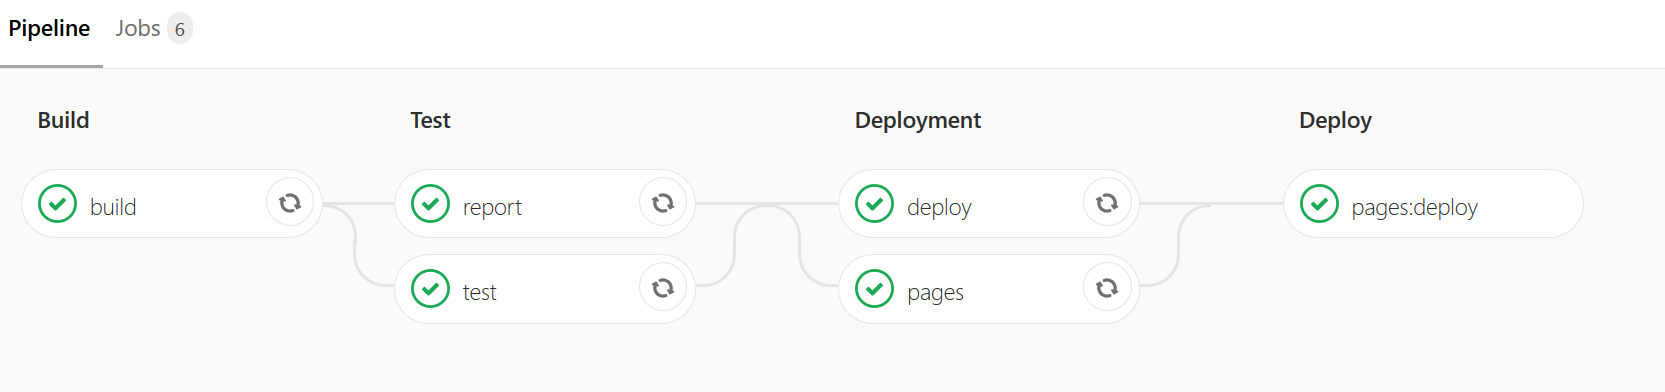
\includegraphics[width=0.9\textwidth]{M3_Pipeline}
 	\caption{Pipeline de GitLab que muestra éxito en todos los trabajos definidos para el proceso de CI/CD}\label{fig:M5_Pipeline}
 \end{figure}
 \FloatBarrier
 
%\todo añadir una captura de pantalla con el badge Heroku del  Readme de Gitlab y explicar como se actualiza cada vez que se realiza un commit. 
%\todo añadir una captura de pantalla con los check verdes en la lista de commit del repositorio de GitLab

\subsubsection{Tokens y variables de entorno}

Para llevar a cabo este proceso de CI/CD, ha sido necesario definir variables de entorno en GitLab que contienen las credenciales o tokens de acceso a Heroku y a Codacy. Esto se realiza desde la ventana de Configuración-CI/CD en la parte de `\textit{Variables}' como se muestra en la Fig. \ref{fig:M5_GitLab_Variables}.

\imagen{M5_GitLab_Variables}{Variables del entorno de ejecución de GitLab}

En el apartado anterior se vé un fragmento de código en el que se utilizan dos de las tres variables que se han definido y se ven en la Fig. \ref{fig:M5_GitLab_Variables}: \textit{\$CODACY\_PROJECT\_TOKEN} y \textit{\$CODACY\_API\_TOKEN}. La otra variable (\textit{HEROKU\_API\_KEY}) se utiliza indirectamente en la actividad de \textit{deploy} de la etapa de \textit{deployment}. Esta no se muestra en el script que define la actividad, sin embargo, fallaría la ejecución de la actividad si no se hubiera definido esta variable.

Estos tokens permiten conectarse a herramientas como Codacy o Heroku ya sea para iniciar sesión o para acceder directamente a un proyecto definido dentro de esas herramientas sin necesidad de tener que tener que iniciar sesión manualmente mediante usuario y contraseña. Esto permite automatizar las tareas que requieran iniciar sesión en herramientas de este tipo. Por ejemplo \textit{\$CODACY\_PROJECT\_TOKEN} es el token que permite acceder al proyecto correspondiente en Codacy y \textit{\$CODACY\_API\_TOKEN} permite utilizar Codacy con una sesión sin tener que iniciar sesión. El primero se obtuvo al configurar la cobertura de código en Codacy y el segundo desde la configuración de la cuenta de usuario en Codacy, en la pestaña `\textit{API Tokens}', se puede generar varios.

\subsubsection{Badges}

Los badges son distintivos o placas que se agregan el el fichero \textit{README} o en el lugar que se permita (admiten varios formatos como Markdown, HTML, Textile, AciiDoc, etc) y aportan información sobre el estado de ciertas características del proyecto tras el último commit como el resultado del pipeline de una actividad de CI/CD, la revisión de calidad, la revisión de cobertura, el estado del despliegue, etc.

En la Fig. \ref{fig:M5_GitLab_Badges_Readme} se muestran los badges que se han definido en el fichero README.md del proyecto. Los badges constan de tres partes:
\begin{itemize}
	\tightlist
	\item Nombre del badge
	\item Imagen en formato \textit{.svg} asociada al estado del atributo que evalúa el badge y ofrecida por el proveedor de la información
	\item Enlace al que redirige al clicar sobre él. Normalmente una página que complete la información que ofrece el badge.
\end{itemize}
En Markdown la sintaxis es la siguiente:

\begin{minipage}{\linewidth}
{\tiny
\begin{lstlisting}[breaklines]
...
[![nombre-del-badge](URL-de-la-imagen)](URL-del-link)
...		
\end{lstlisting}
}
\end{minipage}
, mientras que en HTML sería:

\begin{minipage}{\linewidth}
{\tiny
\begin{lstlisting}[breaklines]
...
<a href="URL-del-link"><img src="URL-de-la-imagen"/></a>
...		
\end{lstlisting}
}
\end{minipage}

\imagen{M5_GitLab_Badges_Readme}{Badges definidas en el fichero README.md del repositorio del proyecto}

En el proyecto se han definido cuatro badges:
\begin{itemize}
	\item \textit{\textbf{Pipeline}}. Muestra la información del último \textit{pipeline} del proyecto ejecutado en GitLab: en ejecucion (\textit{running}), ejecutado correctamente (\textit{passed}), o ejecutado con fallos (\textit{failed}). El proveedor de la imagen y de la información es GitLab y enlaza con el último \textit{pipeline} del proyecto.
	
	\item \textit{\textbf{Code Quality}}. Muestra la calificación de calidad de código que da Codacy al proyecto y enlaza a la página del proyecto en Codacy.
	
	\item \textit{\textbf{Coverage}}. Muestra el porcentaje de cobertura de instrucciones de las pruebas que se realizan durante la ejecución del \textit{pipeline} de GitLab y enlaza a la página del proyecto en Codacy. El dato es recogido durante la actividad \textit{report} de la fase de \textit{test} del \textit{pipeline}.
	
	\item \textit{\textbf{Coverage}}. Debido a problemas con Codacy, se ha decidido poner otro badge de cobertura. Esta vez se obtiene la información directamente desde el pipeline del último commit del repositorio del proyecto. Y enlaza a un informe que genera JaCoCo en formato HTML y que es publicado en el mismo repositorio del proyecto.
\end{itemize}

\subsection{Pruebas unitarias automáticas con JUnit y GitLab}

Para la automatización de la fase de pruebas se han utilizado las herramientas JUnit, Maven y los \textit{pipelines} GitLab. 

JUnit es un framework que permite desarrollar pruebas unitarias sobre el código desarrollado. Además, dispone de un motor para la ejecución de las pruebas y la visualización de los resultados.



Otro aspecto destacable es la uso con funciones avanzadas en la implementación de test unitarios. 
Como ejemplo en el siguiente fragmento de código se recoge como parametrizar un test para especificar un ficheros que recojan los múltiples casos de prueba.
De esta forma se simplifica mucho las prueba.
{\tiny 
	\begin{lstlisting}[breaklines]
	
	@ParameterizedTest(name = "Run with User = \"{0}\" and 
	Password = \"{1}\" must throw an exception.")
	@CsvFileSource(resources = "/testConnectUserPasswordWrong.csv", 
	numLinesToSkip = 1, delimiter = ';', encoding = "UTF-8")
	
	public void testConnectUserPasswordWrong(String user, String password){
	assertThrows(RepositoryDataSourceException.class, () -> {
	repositoryDataSource.connect(user, password);},
	getErrorMsg("testConnectUserPasswordWrong", 
	"Wrong user-password should throw an exception"));
	assertEquals(EnumConnectionType.NOT_CONNECTED, 
	repositoryDataSource.getConnectionType(),
	getErrorMsg("testConnectUserPasswordWrong", 
	"Connection type must be 'NOT_CONNECTED'"));
	}
	\end{lstlisting}
}

\begin{minipage}{\linewidth}
	{\tiny
		\begin{lstlisting}[breaklines]
		...
		report:
		stage: test
		script:
		- mvn clean jacoco:prepare-agent install jacoco:report
		- mvn jacoco:report 
		-DdataFile=$CI_PROJECT_DIR/target/jacoco.exec
		- mvn com.gavinmogan:codacy-maven-plugin:coverage 
		-DprojectToken="$CODACY_PROJECT_TOKEN" 
		-DapiToken="$CODACY_API_TOKEN"
		artifacts:
		paths:
		- $CI_PROJECT_DIR/target/reports/jacoco-reports/
		...		
		\end{lstlisting}
	}
\end{minipage}

En el primer comando se instala y se prepara el generador de informes jacoco.exec, con el segundo se genera un informe de cobertura con JaCoCo. El directorio de destino se ha configurado en Maven:

\begin{minipage}{\linewidth}
	{\tiny
		\begin{lstlisting}[breaklines]
		...
		<build>
		<plugins>
		<!-- Coverage -->
		<plugin>
		<groupId>org.jacoco</groupId>
		<artifactId>jacoco-maven-plugin</artifactId>
		<version>0.8.3</version>
		<configuration>
		<outputDirectory>${project.reporting.outputDirec
		tory}/jacoco-reports</outputDirectory>
		<output>file</output>
		<append>true</append>
		<title>Coverage of project: 
		${project.name}</title>
		</configuration>
		...
		</plugin>
		<plugin>
		<groupId>com.gavinmogan</groupId>
		<artifactId>codacy-maven-plugin</artifactId>
		<version>1.2.0</version>
		<configuration>
		<coverageReportFile>${project.reporting.outputDirec
		tory}/jacoco-reports/jacoco.xml</coverageReportFile>
		</configuration>
		</plugin>
		...
		</plugins>
		</build>	
		...
		<reporting>
		<outputDirectory>${project.build.directory}/reports</outputDire
		ctory>
		</reporting>
		...		
		\end{lstlisting}
	}
\end{minipage}
, con el tercer comando se envía el informe generado \textit{jacoco.xml} a Codacy mediante un plugin y los tokens de acceso al proyecto en Codacy.

\subsubsection{Proyectos de pruebas}

\subsection{Pruebas con Tomcat y despliegue automático en Heroku}

-Pruebas de interfaz manuales
-Prueba de despliegue automático

Para las pruebas se disponían de datos de otros repositorios de GitLab que se han presentado como TFG en el Grado de Ingeniería Informática en la 
Universidad de Burgos. Esto ha facilitado en gran medida el trabajo de pruebas. 

Es destacable la funcionalidad de acceso a los repositorios por el concepto de grupo definido en Gitlab. Esto fue posible gracias a que la empresa Hewlett Packard SCDS en su colabaración con TFG con la UBU organiza su propuestas de TFG en GitLab en grupos para organizarlos por cursos académicos.

\subsection{Revisión automática de la cobertura}

\subsubsection{Configuración de la Herramienta Codacy}

Codacy permite llevar una revisión de la calidad de código y de la cobertura de las pruebas.

Para utilizar esta herramienta se debe tener una cuenta. Te permite iniciar sesión con GitHub, Bitbucket o Google. Una vez iniciada sesión te permite añadir proyectos al entorno Codacy. Para añadir proyectos se debe pulsar sobre el botón \textit{Add project} como se muestra en la Fig. \ref{fig:M5_Codacy_ProjectsPage} y te permite importar los proyectos desde GitHub o Bitbucket (hay que solicitar permisos a GitHub o Bitbucket). Nada más añadirlos, realiza un análisis inicial y, posteriormente, realizará un análisis cada vez que se realice un \textit{commit} en GitHub o Bitbucket.

\imagen{M5_Codacy_ProjectsPage}{Página principal de Codacy para la gestión de proyectos}

Para configurar la revisión de cobertura hay que seguir unos pasos más. Desde la página de \textit{Dashboard} del proyecto (ver Fig. \ref{fig:M5_Codacy_Dashboard}) se puede observar el indicador de cobertura con título \textit{Coverage}. En un proyecto nuevo, este indicador no está disponible hasta que se haya configurado la cobertura, en su lugar aparece el siguiente mensaje: ``\textit{Make sure your code is all tested. Set up your coverage here.}'' con un enlace. El enlace lleva a una página con instrucciones para configurar la cobertura. Es diferente para cada lenguaje de programación.

\imagen{M5_Codacy_Dashboard}{Vista Dashboard del proyecto en Codacy}

Para este proyecto, la configuración de cobertura de Codacy se ha realizado de la siguiente manera:
\begin{enumerate}
	\item Para que haya cobertura, se debe implementar una cobertura de pruebas y se deben pasar estas pruebas correctamente.
	
	\item Añadir el proyecto a Codacy, como se ha indicado anteriormente
	
	\item Seguir en cuenta las instrucciones que se mencionan anteriormente teniendo en cuenta que se utiliza el lenguaje Java y buscando en todo momento la posibilidad de integración con Maven. Los pasos siguen a continuación.
	
	\item Configurar el plugin JaCoCo en el proyecto para generar informes de cobertura. Maven puede facilitar este proceso, por lo que incluimos el plugin de JaCoCo en el \textit{pom.xml} de a siguiente manera en la parte de \textit{build}:\\
	{\tiny
		\begin{lstlisting}[breaklines]
		...
		<build>
		...
		<plugins>
		...
		<plugin>
		<groupId>org.jacoco</groupId>
		<artifactId>jacoco-maven-plugin</artifactId>
		<version>0.8.3</version>
		<configuration>
		<outputDirectory>${project.reporting.outputDirectory}/jacoco-reports</outputDirectory>
		<output>file</output>
		<append>true</append>
		<title>Coverage of project: ${project.name}</title>
		</configuration>
		<executions>
		<execution>
		<id>pre-unit-test</id>
		<goals>
		<goal>prepare-agent</goal>
		</goals>
		</execution>
		<execution>
		<id>post-unit-test</id>
		<phase>test</phase>
		<goals>
		<goal>report</goal>
		</goals>
		</execution>
		</executions>
		</plugin>
		</plugins>
		...
		</build>
		...
		\end{lstlisting}
	}
	
	De esta forma se configura el directorio de destino:\\ \textit{\${project.reporting.outputDirectory}/jacoco-reports}, \\el título del informe:\\\textit{Coverage of project: \${project.name}}\\ y dos unidades de ejecución: una para preparar el generador, y otra para generar el informe.
	
	\item Utilizar \textit{codacy-maven-plugin} para enviar el informe de cobertura generado por JaCoCo a Codacy. También se puede añadir el plugin en la parte de \textit{buid} de Maven:
	{\tiny
		\begin{lstlisting}[breaklines]
		...
		<build>
		...
		<plugins>
		...
		<plugin>
		<groupId>com.gavinmogan</groupId>
		<artifactId>codacy-maven-plugin</artifactId>
		<version>1.2.0</version>
		<configuration>
		<coverageReportFile>${project.reporting.outputDirectory}/jacoco-reports/jacoco.xml</coverageReportFile>
		</configuration>
		</plugin>
		</plugins>
		...
		</build>
		...
		\end{lstlisting}
	}
	Para este 
\end{enumerate}

Al gestionar la revisión de calidad por primera vez en este proyecto, Codacy permitía añadir repositorios a partir de su \textit{Git URL}. Esto permitió añadir nuestro proyecto de GitLab al entorno de Codacy. Sin embargo, esta funcionalidad les daba muchos problemas y la acabaron eliminando. Esto paró las revisiones de calidad automáticas de este proyecto.
-Configuración con Codacy
-Problemas con Codacy: porque se obtiene de dos formas diferentes
-Configuración badge GitLab con regex y publicación de informe de JaCoCo

\subsection{Administración de calidad automática con Codacy}
En los últimos sprints, correspondientes a la entrega de prototipos funcionales al tutor,
se definía una tarea para analizar la deuda técnica que indicaba la Codacy.
Se analizaban las tareas de mejoras propuesta por Codacy según su orden de prioridad y se intentaban eliminar.
De esta forma además de aprender de las revisiones automáticas de Codacy se controlaba la deuda técnica, en el prototipo evolutivo.
La valoración final del proyecto ha sido la máxima (A) sin ninguna revivión de calidad de alta prioridad.
%\todo Añadir url de codacy de tu proyecto y una captura de pantalla donde aparezca la A.

-Marca actual
-Ejemplos de correcciones + captura
-Problemas con codacy + soluncion: exportar proyecto a GitHub

\subsection{Despliegue automático con Heroku}

\subsubsection{Configuración de la Herramienta Heroku}

Heroku es una plataforma que permite desplegar una aplicación web en sus servidores. Para ello debes tener una cuenta, crear un pipeline y una aplicación y asociar la aplicación al pipeline. Para desplegarla se ofrecen tres opciones: \textit{Heroku Git}, \textit{GitHub} y \textit{Heroku CLI}.

En este proyecto se ha utilizado Heroku CLI y un plugin para integrarlo con Maven:\\
\begin{minipage}{\linewidth}
	{\tiny
		\begin{lstlisting}[breaklines]
		...
		<build>
		<plugins>
		...
		<!-- Deployment -->
		<plugin>
		<groupId>com.heroku.sdk</groupId>
		<artifactId>heroku-maven-plugin</artifactId>
		<version>2.0.9</version>
		<configuration>
		<appName>evolution-metrics</appName>
		</configuration>
		</plugin>
		</plugins>
		</build>
		...
		\end{lstlisting}
	}
\end{minipage}

En el código anterior se configura el plugin para desplegar en la aplicación con nombre \textit{evolution-metrics}. El comando para  desplegar la aplicación sería \textit{\$ mvn clean heroku:deploy-war}. Sin embargo, para que funcione correctamente se debe iniciar sesión con \textit{\$ heroku login}, que abre el navegador en la página de inicio de sesión de Heroku. De esta forma es imposible desplegar la aplicación automáticamente, para que se pueda desplegar de una forma completamente automática se debe configurar la variable de entorno \textit{HEROKU\_API\_KEY} con el token de acceso \textit{API Key} que se obtiene desde la configuración de la cuenta de usuario. Esta variable se ha definido dentro de las variables de entorno de GitLab de las que se hablaba anteriormente, y el comando de despliegue se ejecuta desde los \textit{pipelines} gracias a la actividad \textit{deploy} de la etapa \textit{deployment} definidas en el fichero \textit{.gitlab-ci.yml}
\section{API de GitLab}

GitLab ofrece un API \footnote{\url{https://docs.gitlab.com/ee/api/}} para poder desarrollar aplicaciones que integren funcionalidades de GitLab. En este proyecto se ha utilizado este API para establecer una conexión a GitLab y poder calcular métricas de los repositorios que aloje.

En lugar de trabajar directamente con GitLab API, se decidió usar un \textit{framework} en Java. Se tenían dos opciones:
\begin{itemize}
	\item \textit{timols/java-gitlab-api} \footnote{\url{https://github.com/timols/java-gitlab-api}}. La documentación es bastante pobre y la evolución del proyecto software estaba parada o no evolucionaba bien, tenían demasiadas incidencias abiertas y no ofrecía gran parte de la funcionalidad que aportaba GitLab API.
	\item  \textit{gitlab4j/gitlab4j-api} \footnote{\url{https://github.com/gitlab4j/gitlab4j-api}}. Es un proyecto bastante decente y, a día de hoy, sigue creciendo. Tiene buena documentación,  un alto porcentaje de incidencias cerradas, un gran número de releases, y evolución constante. 
\end{itemize}

La decisión era clara y \textit{gitlab4j/gitlab4j-api} es con el que se ha desarrollado este proyecto y ha permitido obtener todos los datos de los repositorios de GitLab para calcular todas las métricas. Para utilizar este API solo ha sido necesario incluirlo entre las dependencias del proyecto en el fichero \textit{pom.xml}. 

\section{Diseño extensible}

\section{Interfaz gráfica: Vadin}
-Ventajas e inconvenientes
-Ejemplo de uso
-Framework de pestañas de conexión y gestión de repos
-Configuración en maven adicional para poder ser utilizado en internet explorer
-Díalogo: problemas y solución
-Designer
-Despliegue en tomcat, falta de xml, porque no jetty
-No Adaptativo